\documentclass{article}

\usepackage{graphicx}
\usepackage{tikz}
\usepackage{tikzsymbols}
\usetikzlibrary{calc}
\usepackage{float}
\usepackage{pdflscape}
\usepackage{geometry}

\def\centerarc[#1](#2)(#3:#4:#5){\draw[#1] ($(#2)+({#5*cos(#3)},{#5*sin(#3)})$) arc (#3:#4:#5);}

\pagestyle{empty}
\begin{document}
    \centering
	\begin{figure}[H]
		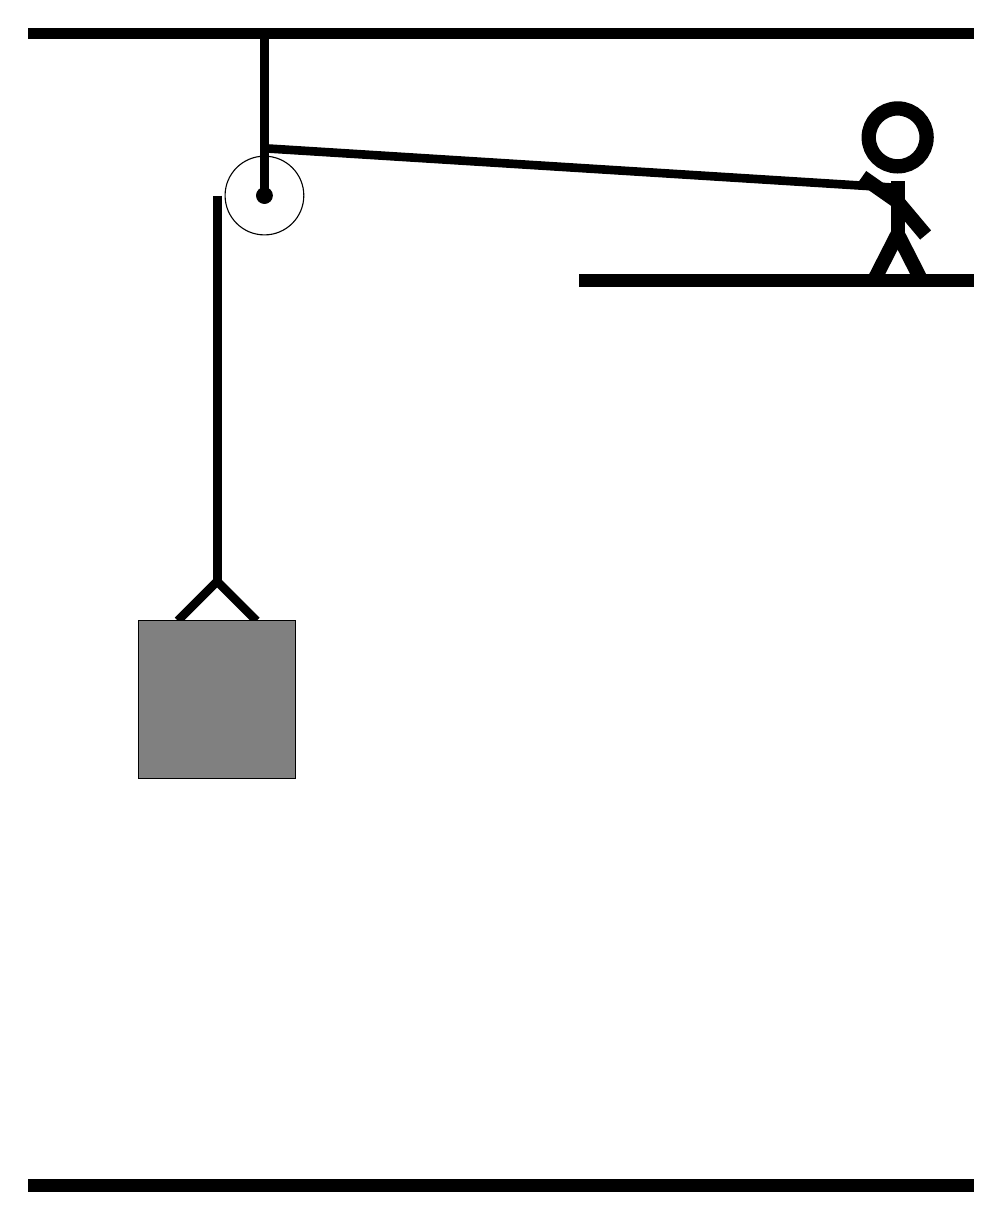
\begin{tikzpicture}
			%%%%% START %%%%%
			\def\a{11.5}
			\def\radlg{0.5}
			\def\radrp{0.6}
			\def\radsm{0.1}
			\def\yone{\a-2}
			\def\xone{1}
			\def\xtwo{3.5}
			\def\xthree{4.7}
			\def\ythree{-1}
			\def\dxtwo{9}
			\def\dx{9}
			\def\dy{\a-2}
			\def\dw{1.75mm}
			\def\hlena{\a*0.6}
			\def\width{1.1mm}
			
			\draw[fill=black] (-2,\a) rectangle (10,\a+0.125);

			\draw (\xone,\yone) circle (\radlg);
			\draw[fill=black] (\xone,\yone) circle (\radsm);
			\draw[line width=\width] (\xone,\a) -- (\xone,\yone);
			
			\draw[line width=\width](\xone-0.5-\radrp,\a-\hlena-0.5) --  (\xone-\radrp,\a-\hlena) -- (\xone+0.5-\radrp,\a-\hlena-0.5);			
			\draw[fill=black!50] (\xone-1-\radrp,\a-\hlena-0.5) rectangle (\xone+1-\radrp,\a-\hlena-2-0.5); 
			
			\draw[line width=\width](\xone-\radrp,\yone) -- (\xone-\radrp,\a-\hlena);
			\centerarc[line width=\width](\xone,\yone)(90:180:\radrp)
			\draw[line width=\width](\xone,\yone+\radrp) -- (\dx,\dy+.1);

			\node at (\dx,\dy) {\Strichmaxerl[10][-35][-50]};
			\draw[fill=black] (5,\a-3) rectangle (10,\a-3.15);
			
			\draw[fill=black] (-2,-3) rectangle (10,-3.15);
			%%%%% END %%%%%
		\end{tikzpicture}
	\end{figure}
\end{document}